\chapter{Struktura techniczna aplikacji}
\label{cha:budowaSystemuIstruktura}

Głównym celem było stworzenie przejrzystej i logicznie podzielonej architektury, która ułatwia rozwój, testowanie i dalsze utrzymanie.System został podzielony na trzy cześći, gdzie wyraźnie oddzielono warstwę prezentacji (GUI), logiki biznesowej oraz dostępu do danych. Struktura kodu została podzielona na klasy odpowiadające poszczególnym funkcjom aplikacji.
% ------------------------------------------------------------------------
\section{Projekt bazy danych}
System korzysta z relacyjnej bazy danych MySQL.Tabele są ze sobą powiązane kluczami obcymi, co zapewnia spójność danych.Poniżej przedstawiono diagram ERD obrazujący relacje między tabelami w bazie danych. Diagram pokazuje powiązania między użytkownikami, sprzętem, rezerwacjami i wypożyczeniami. Dzięki temu możliwe było zaprojektowanie struktury danych, która wspiera wszystkie funkcje aplikacji.

\begin{figure}[H]
    \centering
    \includegraphics[width=\linewidth]{figures/schematBazyDanych.jpg}
    \caption{Diagram ERD przedstawiający relacje w bazie danych.}
    \label{fig:diagram_erd}
    \small{Źródło: Opracowanie Własne}
\end{figure}
\clearpage
\section{Architektura i hierarchia klas}
Aplikacja została zaprojektowana w architekturze trójwarstwowej. Każda z nich pełni odrebną funkcję:
\begin{enumerate}
    \item Warstwa prezentacji: formularze graficzne (GUI) – klasy dziedziczące po JFrame, takie jak RezerwacjaSprzetuForm, ProfilUzytkownikaForm, AdminPanelForm;
    \item Warstwa logiki aplikacji: klasy odpowiedzialne za przetwarzanie danych i decyzje (np. ZarzadzanieRezerwacjami, DodawanieEdycjaSprzetu);
    \item Warstwa dostępu do danych: DatabaseConnection i zapytania SQL realizowane przez PreparedStatement.
\end{enumerate}

\subsection{Diagram UML klas dziedziczących}
\begin{figure}[H]
    \centering
    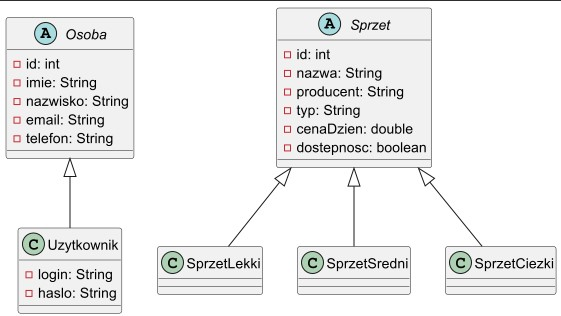
\includegraphics[width=\linewidth]{figures/dziedziczenie.jpg}
    \caption{Diagram UML przedstawiający relacje klas dziedziczących.}
    \label{fig:diagramDziedziczacych_uml}
    \small{Źródło: Opracowanie Własne z wykorzystaniem PlantUML}
\end{figure}
\clearpage


